
\documentclass[11pt]{article}

% Language setting
% Replace `english' with e.g. `spanish' to change the document language
\usepackage[english]{babel}
\usepackage[margin=1in]{geometry} 
\usepackage{amsmath,amsthm,amssymb,scrextend}
\usepackage{fancyhdr}
\pagestyle{fancy}

\newcommand{\cont}{\subseteq}
\usepackage{tikz}
\usepackage{pgfplots}
\usepackage[export]{adjustbox}
\usepackage{amsmath}
\usepackage[mathscr]{euscript}
\let\euscr\mathscr \let\mathscr\relax% just so we can load this and rsfs
\usepackage[scr]{rsfso}
\usepackage{amsthm}
\usepackage{amssymb}
\usepackage{multicol}
\usepackage[colorlinks=true, pdfstartview=FitV, linkcolor=blue, citecolor=blue, urlcolor=blue]{hyperref}
\usepackage{listings}
\definecolor{codegreen}{rgb}{0,0.6,0}
\definecolor{codegray}{rgb}{0.5,0.5,0.5}
\definecolor{codepurple}{rgb}{0.58,0,0.82}
\definecolor{backcolour}{rgb}{0.95,0.95,0.92}

\lstdefinestyle{mystyle}{
    backgroundcolor=\color{backcolour},   
    commentstyle=\color{codegreen},
    keywordstyle=\color{magenta},
    numberstyle=\tiny\color{codegray},
    stringstyle=\color{codepurple},
    basicstyle=\ttfamily\footnotesize,
    breakatwhitespace=false,         
    breaklines=true,                 
    captionpos=b,                    
    keepspaces=true,                 
    numbers=left,                    
    numbersep=5pt,                  
    showspaces=false,                
    showstringspaces=false,
    showtabs=false,                  
    tabsize=2
}

\lstset{style=mystyle}

\DeclareMathOperator{\arcsec}{arcsec}
\DeclareMathOperator{\arccot}{arccot}
\DeclareMathOperator{\arccsc}{arccsc}
\newcommand{\ddx}{\frac{d}{dx}}
\newcommand{\dfdx}{\frac{df}{dx}}
\newcommand{\ddxp}[1]{\frac{d}{dx}\left( #1 \right)}
\newcommand{\dydx}{\frac{dy}{dx}}
\let\ds\displaystyle
\newcommand{\intx}[1]{\int #1 \, dx}
\newcommand{\intt}[1]{\int #1 \, dt}
\newcommand{\defint}[3]{\int_{#1}^{#2} #3 \, dx}
\newcommand{\imp}{\Rightarrow}
\newcommand{\un}{\cup}
\newcommand{\inter}{\cap}
\newcommand{\ps}{\mathscr{P}}
\newcommand{\set}[1]{\left\{ #1 \right\}}
\newtheorem*{sol}{Solution}
\newtheorem*{claim}{Claim}
\newtheorem{problem}{Problem}

\newcommand{\HRule}{\rule{\linewidth}{0.5mm}}
\newcommand{\codeword}[1]{\texttt{\textcolor{blue}{#1}}}

\setlength{\columnsep}{1cm}

\begin{document}
 
% EVERYTHING ABOVE THIS LINE IS JUST PREABLE, NO NEED TO MESS WITH IT.__________________________________________________________________________________________
%

\begin{titlepage}
  \begin{center}
    % logo
    
\includegraphics[width=0.5\textwidth]{figures/SoC-CU-Orange-and-Purple.png}~\\[2cm]

    \textsc{\Large CPSC 4300/6300 \\ Applied Data Science \\ Fall 2023}\\[1cm]


    \HRule \\[0.4cm]
    {\large \bfseries Course Project: Final Project Submission\\ Detecting working patterns from online workers and \\ predicting task completion. \\[0.4cm]}
    \HRule \\[2cm]
    
    \large\textbf{Students:}\\
    STEPHEN BECKER, DAVID CROFT, ZACHARY TRABOOKIS \\ School of Computing \\ College of Engineering, Computing and Applied Sciences \\ 
    Clemson University\\[1cm]

    \large\textbf{Instructor:}\\
    DR. NINA HUBIG  \\ School of Computing \\ College of Engineering, Computing and Applied Sciences \\ 
    Clemson University\\[1cm]

    \vfill

    {\large \today}

  \end{center}
\end{titlepage}

\lhead{CPSC 4300/6300}
\chead{Becker, Croft, Trabookis}
\rhead{\today}
 
% \maketitle

\section{Introduction}

\begin{multicols}{2}

The rise of AI technologies has created a vast amount of work for independent workers. These jobs include activities such as image, text, and audio annotation, as well as audio transcription, completing surveys, and many other activities. The crowdsourcing platforms (i.e., Amazon Mechanical Turk (MTurk), Yandex Toloka, etc.) offer microtasks to online workers from all over the world. This type of work is considered invisible work since it is not regulated, and few people know about it. The working patterns of these workers can be studied by analyzing telemetry data from workers completing tasks. This project aims to understand the working patterns of these workers and build AI models able to predict the activities they will take and finish. In particular, we are looking to use a machine learning model to help a crowd worker determine whether or not they should take a task based on if they would complete or not complete an individual task based on previous information and data training.

\subsection{Motivation}
Crowd workers spend additional time outside just completing the project task, which is not accounted for in the original requester’s estimated labor cost and duration, and can be identified as invisible work. The predicted completed task output from our model can be used by a crowd worker when deciding whether to take on a new task or not. The completed task metric could be provided on a project task dashboard for the crowd worker to review prior to selecting their next task to start. This metric along with other invisible labor metrics, not identified by this paper, can be used to alter the requester task award costs or estimate time to complete for a particular task. It’s important that the crowd worker gets fair compensation for the additional unpaid invisible labor work when completing a requester task. It’s important to understand that evaluation of this invisible work could help change the wage for the crowd workers or provide a fair compensation estimate for a new task that a requester may create on the crowdsourcing platform.  

\subsection{Dataset}
A research article titled \textit{Quantifying the Invisible Labor in Crowd Work}. \cite{toxtli2021} provided the original telemetry dataset which came from extending the Turkenator Chrome Extension (plugin) to collect information necessary to report on working and  invisible labor events. \cite{toloka-web-extension-github} The plugin helps (1) detect when a worker is doing invisible labor or when they are doing paid work; and (2) measures how much time a worker invests in each of these two activities. \cite[p.~4]{toxtli2021}

The plugin includes a "background process that detects the different browser events that happen on MTurk (e.g., that the worker visited another page on MTurk, or that she started typing, or began a new HIT). The page crawler detects the current MTurk domain page that the worker is on, as well as the status of the page (e.g., that the page is loaded, active, inactive, or closed). The background process focuses on detecting the human intelligence tasks (HITs) that the worker is currently doing and identifying which she has finished. In order to accomplish this, the background process polls workers’ task queues on MTurk every 30 seconds. From the task queue, the background process obtains the metadata and status of all the HITs the worker has accepted to do. Notice that the page crawler is the primary element that we use to detect whether the worker is completing paid labor or invisible labor. The background process helps our plugin to be able to better detect when the worker is completing HITs." \cite[p.~5]{toxtli2021}

The datasets that we are examining are from Amazon Mechanical Turk (MTurk) and Toloka Yandex. They observe individuals and the actions they perform while working tasks, storing them as individual events, on their respective platforms. Combined they consist of 302 unique individuals contributing 12,401,997 individual actions/events towards this dataset. There is over 4 days worth of information in the MTurk dataset; whereas, Toloka has over 43 days worth of information. Both datasets have 10 columns worth of quantitative and numerical data which includes event id’s, page urls, page actions, API calls, task status, epoch timestamp, working status, person id, and two other columns that contain unusable data. Our next step was to condense our dataset and to make new columns that contained more relevant data to our problem, especially since the API calls had a bunch of useful information in the API json request. 

\end{multicols}

\subsection{List of Variables}
The dataset did not include column names and no description was provided. After locating the research paper and talking with Carlos Toxtli through email, we were able to identify these names and descriptions. If we didn't have this initial paper it would have been hard for us to figure out exactly what was going on with the dataset provided.
\begin{itemize}
    \item \textbf{c1 (id):} continuous id of the event generated by the Chrome Extension. \cite{toloka-web-extension-github}
    \item \textbf{c2 (current):}  url, site visited by the worker (while working)
    \item \textbf{c3 (event):} categorical, 18 values
    \begin{itemize}
        \item The web browser plugin recorded multiple events, the most relevant is \codeword{PAGE\_LOAD}, other events can provide repetitive information.
        \begin{lstlisting}[language=Python, caption=Chrome Plugin: 'events' value.]
(['PAGE_LOAD', 'PAGE_BLUR', 'TAB_CHANGE', 'PAGE_FOCUS', 'PAGE_CLICK', 'PAGE_SCROLL', 'PAGE_LAST', 'PAGE_CLOSE', 'INTERNALURL', 'PAGE_KEY', 'PAGE_INACTIVITY', 'TAB_CLOSED', 'EXTERNALURL', 'PAGE_REACTIVATE', 'SYSTEM_DISABLED_WORKING', 'SYSTEM_ENABLED_WORKING', 'SYSTEM_ENABLED', 'SYSTEM_DISABLED'])
\end{lstlisting}
    \end{itemize}
    \item \textbf{c4 (extra):} JSON object – may include NaN values
    \\ It provides the specifics of the tasks, it only has values for certain events. The following is a list of values used in the final cleaning csv.
    \begin{itemize}
        \item \textbf{task\_id:} continuous id of the task that the worker accepts to work on.
        \item \textbf{requester\_name company:} name who created the task to be completed by the worker.
        \item \textbf{assignment\_duration\_in\_seconds:} number or seconds estimated to complete the project.
        \item \textbf{project.assignable\_hits\_count:} number of human intelligence tasks (HITs) the worker must complete for the project before they can claim completion.
        \item \textbf{project.monetary\_reward.amount\_in\_dollars:} US dollar award amount after the project has been completed by the worker.
    \end{itemize}
    \item \textbf{c5 (platform):} categorial, 5 values
    The work platform in which the worker was working on (it is usually constant). Because we were focused on reading AWS Mechanical Turk data this value stated \codeword{MTURK}.
    \begin{lstlisting}[language=Python, caption=Chrome Plugin: 'platform' value.]
['OTHER', 'MTURK', 'FIVERR', 'UPWORK', 'FREELANCER']
\end{lstlisting}
    \item \textbf{c6 (skip):} categorial, 2 values (0, 1) – may include NaN value \\
    After talking with Carlos Toxtli, he mentioned that he didn't remember the purpose of this field. This field was unused.
    \item \textbf{c7 (subtype):} categorial, 29 values
    \begin{itemize}
        \item It defines if a worker is listing the tasks available, if a task just started, or if a task was completed (submitted)
        \item \codeword{FINISHED\_TASK == TASK\_SUBMITED} both refers to task completed (submitted is when it was recently submitted and finished when the next URL was loaded)
        \item \codeword{TASK\_RETURNED} When the worker decided not to work on a task.
    \end{itemize}
    \begin{lstlisting}[language=Python, caption=Chrome Plugin: 'subtype' value.]
['OTHER', 'TASK_STARTED', 'ADDED_TASK', 'TASK_SUBMITED', 'FINISHED_TASK', 'TASKS_LIST', 'WORKER_DASHBOARD', 'UNKNOWN', 'TASK_FRAME', 'TASK_PREVIEW', 'TASK_INFO', 'TASK_RETURNED', 'PLATFORM_LOGIN', 'TASK_QUEUE', 'TASK_SKIP', 'WORKER_EARNINGS_DETAILS', 'TASK_TIMEOUT', 'WORKER_EARNINGS', 'WORKER_QUALIFICATIONS', 'TASKS_PER_REQUESTER', 'MESSAGES_SEND', 'TASKS_LIST_FILTER', 'WORKER_QUALIFICATIONS_PENDING', 'TASKS_PREVIEW', 'PLATFORM_HELP', 'TASKS_PROJECTS', 'TASKS_DETAILS', 'MESSAGES_READ', 'TASKS_APPLY']
\end{lstlisting}
    \item \textbf{c8 (time):} continuous, datetime (milliseconds), 1970 start date Unix Time (Week, Month, Day, Hours, Minutes, Seconds).\\ \\
    This is a timestamp in milliseconds (Example: \codeword{1588994235725}). We had to convert to a datetime format with day, month, year, hour, minute, second. This datetime value represents when the Chrome Extension \cite{toloka-web-extension-github} event log was occurred (Example \codeword{2020-05-09T23:31:31.151000}).
    \item \textbf{c9 (type):} categorial, 10 values \\
    It identifies if at that time the worker was working, communicating by sending messages in the platform, searching for tasks, visiting their profile. There are other types that mean that the workers changed the CONFIG of the Chrome Extension \cite{toloka-web-extension-github} or the API of Toloka retrieved new tasks.

    The research paper mentioned that 
    \begin{lstlisting}[language=Python, caption=Chrome Plugin: 'type' value.]
['OTHER', 'WORKING', 'LOGS', 'SEARCHING', 'PROFILE', 'UNKNOWN', 'REJECTED', 'COMMUNICATION', 'LEARNING', 'PROPOSAL']
\end{lstlisting}
    \item \textbf{c10 (user):} categorical, 120 values unique \\
    The worker id performing the crowdwork task.
    \item \textbf{c11:} Not relevant (an activity was taken after being recommended)
    \item \textbf{c12:} Not used
\end{itemize}

\section{Summary of Exploratory Data Analysis (EDA)}

\subsection{Data Processing and Cleaning}
The original MTurk dataset was generated from a Turkenator Chrome Extension (plugin) that was modified to collect information necessary to report on working and invisible labor events. We noticed that the events included \codeword{(user\_id, task\_id)} fields that we could leverage to group events together for our final feature set; designated values \codeword{(ADDED\_TASK, FINISHED\_TASK)} from a subtype event field provided ranges for start/stop for a given task. We had to filter out tasks that did not include both an \codeword{(ADDED\_TASK, FINISHED\_TASK)} entries as this would show incomplete information. An event timecode field was provided in milliseconds which needed to be converted to a datetime format to easily identify when an event occurred; this field was important for sorting events in a chronological order of occurrence and was necessary when aggregating the duration and count totals correctly. Flattening of an event details JSON field was needed to retrieve additional data fields \codeword{(task\_id, requester\_name\_company, assignment\_duration\_seconds, \\project.assignable\_hit\_counts, project.monetary\_reward\_in\_dollars)}. We calculated new fields for our feature set to include total, working, and invisible labor count and duration in seconds; adjusted monetary reward in dollars from the working + invisible labor; completed\_task (yes/no). Processing and cleaning this data was not easy because it relied upon internal knowledge about how this data was collected through the Chrome plugin, and also figuring out how to best group individual event recordings for a task was a challenge because we had to figure out when they started and stopped.

$$\textbf{Task Pay Rate (dollars)} = \frac{\text{Task Monetary Reward (dollars)}}{\text{Task Estimate Duration (seconds)}}$$

\begin{multline*}
\textbf{Adjusted Monetary Reward (dollars)} = \text{Task Monetary Reward (dollars)} \\ + \text{Task Pay Rate (dollars)} \times \\ (\text{Working Labor Duration (seconds)} + \text{Invisible Labor Duration (seconds)})
\end{multline*}

\subsection{Data Visualization \& Key Predictors}
The projected model that will use this dataset will be constructed to predict the completion status of a task, given selected features associated with a task. As described before, completion status is a binary field, where 1 corresponds to a completed task, and 0 corresponds to a task that was never finished. As such, a classification model will be used to determine this discrete outcome with two options. Figure 1 gives a glance at the distribution of completed tasks for a subset of our cleaned, task-grouped dataset.

Due to lack of familiarity with this type of dataset, an EDA had to be performed to understand how the given features correspond with our outcome, whether a task was completed or not. Some of the features were seemingly too irregular or unrelated to task completion to use in our model, like the total time allotted by a requester for the task. However, there were three very promising features that were selected as key predictors because they showed an interesting relationship when plotted against each other for classification: monetary reward for the completion of the task, number of human intelligence subtasks ("HITs") for the task, and total number of events recorded which includes both invisible labor events and visible labor events. Figure 4 has several plots showing how these key predictors relate to one another, with orange and blue legends corresponding to whether the task was completed or not, respectively. Figure 2 and 3 show how the task monetary reward relates to the task completion status.

\begin{figure}[hbt!]
  \centering
  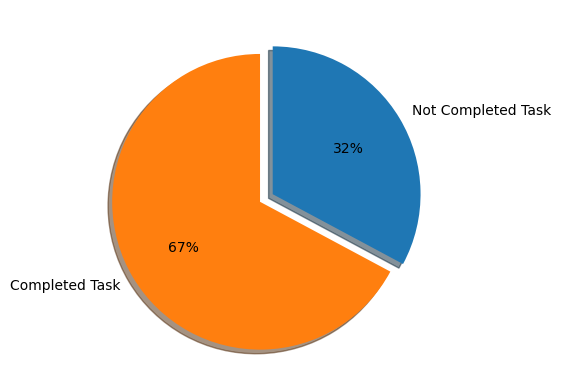
\includegraphics[width=425pt]{figures/distribution-completed-tasks-pie-chart}
  \caption{Distribution of Completed Task Status values.}
\end{figure}

\clearpage

\begin{figure}[hbt!]
  \centering
  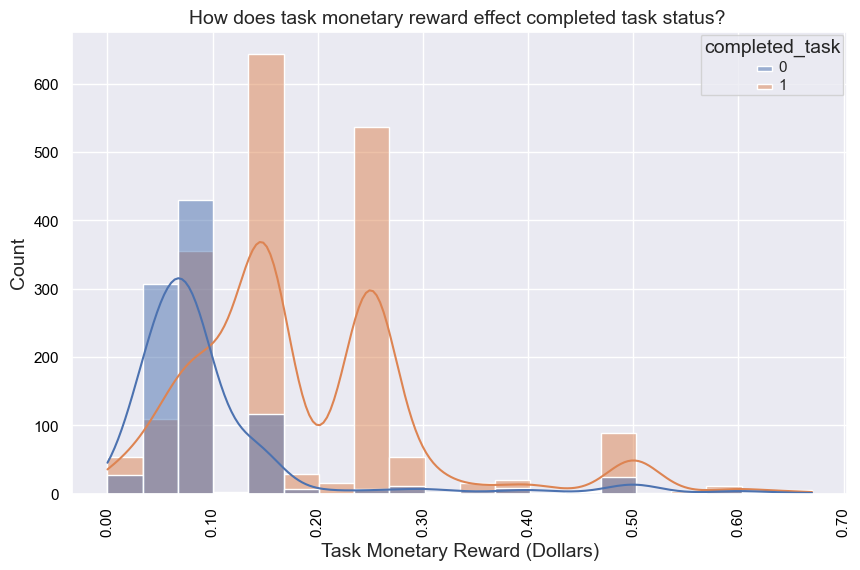
\includegraphics[width=420pt]{figures/task-monetary_reward_in_dollars-vs-completed_task-histogram}
  \caption{Histogram - Count of Task Monetary Reward for Task Completion Status.}
\end{figure}

\begin{figure}[hbt!]
  \centering
  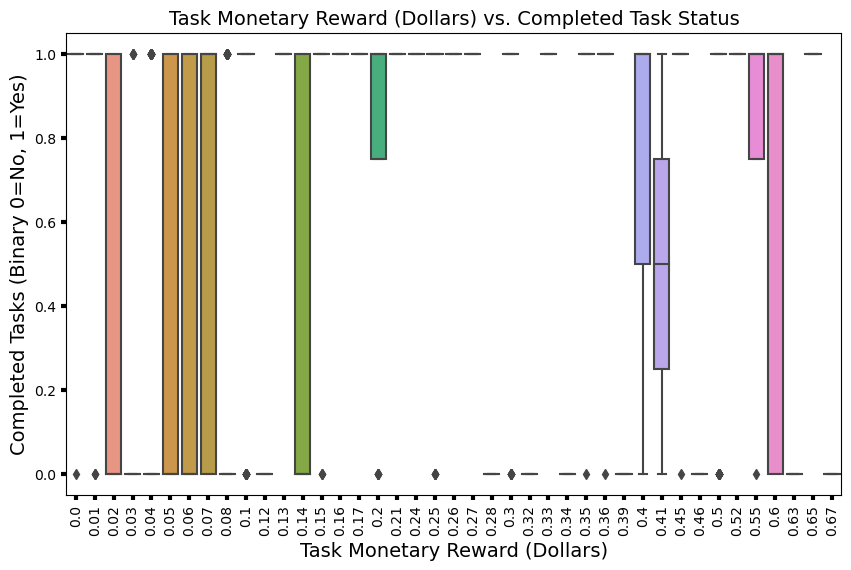
\includegraphics[width=420pt]{figures/task-monetary_reward_in_dollars-vs-completed_task-boxplot}
  \caption{Box Plot - Task Monetary Reward for Task Completion Status.}
\end{figure}

\clearpage

\begin{figure}[hbt!]
  \centering
  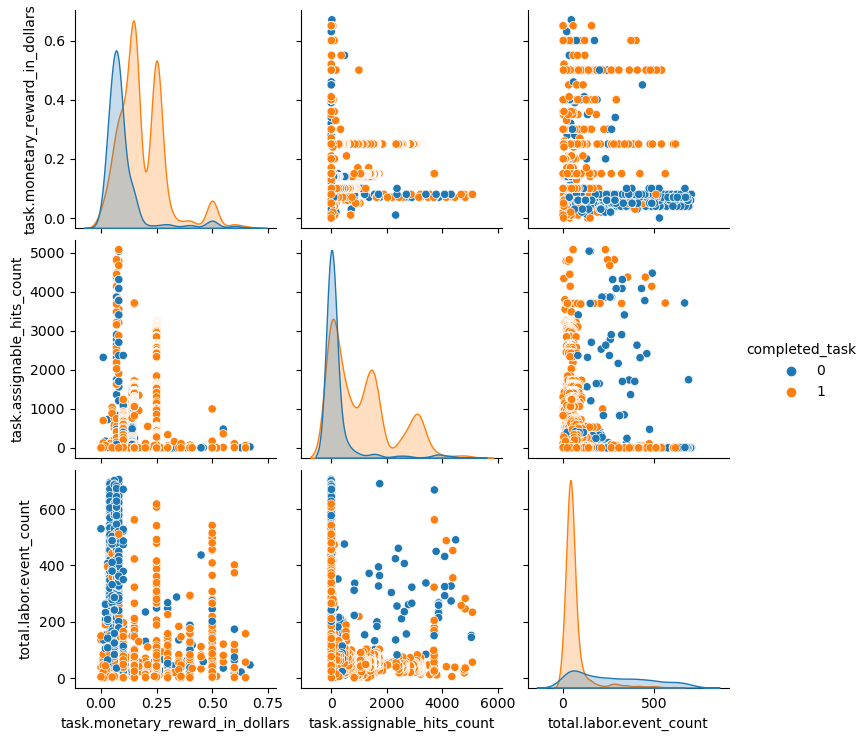
\includegraphics[width=\linewidth]{figures/sns-pairplot}
  \caption{Seaborn Pairplot for model predictors.}
\end{figure}

\section{Model Choice \& Justification}

The response variable for our model to predict is the binary completion status of a task accepted by a crowdsource worker: 1 for a task that is completed, 0 for a task that was not completed. To predict this binary outcome, we must select a classification model. We chose to look into k-Nearest Neighbors (kNN) and Support Vector Machine (SVM) models for this prediction output.

\subsection{K-Nearest Neighbors (kNN)}
This model was chosen over a linear regression classification model because, in our EDA, we found that much of our data was tightly clustered around lower values, and was not easily linear separable. The initial model has a k-value of k = 3 to avoid any erroneous classifications that fall outside the tight cluster groups in the plot of key predictors.

%\begin{multicols}{2}
\subsubsection{Model Analysis}
%\begin{multicols}{2}
For the binary classification model, a confusion matrix is an appropriate visualization to demonstrate how the model performs on test data. Figure 5 demonstrates how the model performed on a test subset of the data using a matrix, where correctly classified predictions are in the top left and bottom right squares, and misclassified predictions are in the other squares. A confusion matrix may be supplemented with classification metrics to understand the rate of model error: accuracy, the percentage of all correct classifications, precision, the percentage of correct positive classifications, and recall, the percentage of positive classifications identified by the model.

\begin{figure}[hbt!]
  \centering
  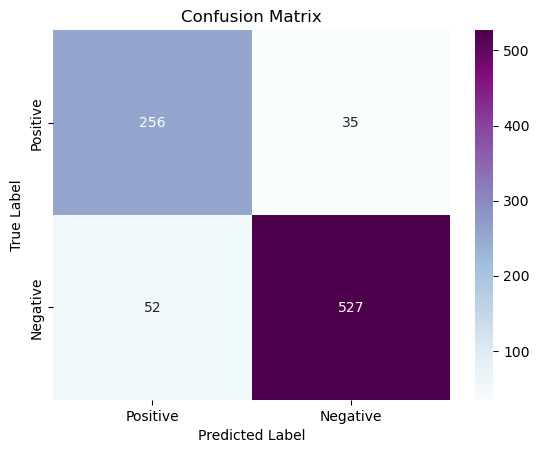
\includegraphics[width=375pt]{figures/confusion-matrix-knn}
  \caption{Confusion Matrix: K-Nearest Neighbors.}
\end{figure}

\subsubsection{Model Evaluation}
Table 1 shows the accuracy, precision, and recall of the model, where the closer the value is to one, the less error the model had in predicting task completion. This means of error rate evaluation serves a binary classifier the best because it puts the rate of successful distinction between two choices into perspective, with respect to different measures of success. For example, if our goal of error analysis is to simply evaluate the rate of any successful classifications, accuracy serves best, but if we are most concerned with correctly identifying positive cases, we should look at recall.

\begin{table}[hbt!]
   \large
   \centering
   \begin{tabular}{lccr}
   \hline
   \textbf{Evaluation Metric} & \textbf{Value} \\ 
   \hline
   Accuracy & 0.9  \\
   Precision & 0.8311688311688312  \\
   Recall & 0.8797250859106529  \\
   \end{tabular}
   \caption{kNN Evaluation Metrics} 
%   \label{tab:example}
\end{table}


Based on the classification metrics obtained with testing data, 90\% of the time our kNN model appears to correctly identify whether or not a task will be completed. Relatively speaking, this is a pretty good chance of identification, given the confusing, clustered nature of the data shown in the EDA. The lowest classification metric is precision, which means that the model has the highest rate of error when it makes a positive classification prediction. Nonetheless, this is still greater than 80\%, which is still significant, given the density of the plots of the dataset's features. Overall, for an initial model, it does a fairly adequate job of fitting the data and correctly classifying unseen data.
%\end{multicols}

\subsection{Support Vector Machine (SVM)}
The first model chosen for classification was a K-Nearest Neighbors model, which is a relatively simple method where an observation is classified based on the category of close data points in the training set. For our second model, we decided to go with a support vector machine for classification, which attempts to classify data by splitting and spacing them along a decision boundary. We chose this model because it offered a more nuanced approach to classifying a dense dataset, and the high dimensionality of our inputs would not be a problem.

%\begin{multicols}{2}
\subsubsection{Model Analysis}
The model includes different types of kernels (algorithms that determine the similarity between input vectors). We chose a ‘rbf’ or Radial Basis Function (RBF) kernel because the input data had more clustered points from our EDA and was non-linear. We left the hyperparameter ‘C’, which controls the trade-off between the insensitive and sensitive loss, at the default of 1.0 value. The smaller the ‘C’ means that the model will be more lenient in allowing larger errors and larger value means that the model will minimize the insensitive loss more. Table 2 shows the score (mean accuracy), accuracy, precision, recall, and F1-Score (harmonic mean of precision and recall) of the SVM model, where the closer the value is to one, the less error the model had in predicting task completion. As shown in Table 2, our choice of an rbf kernel is validated since the SVM gives the best accuracy, precision, recall, and F-1 score of all kernels.

%\begin{figure}[h]
%  \centering
%  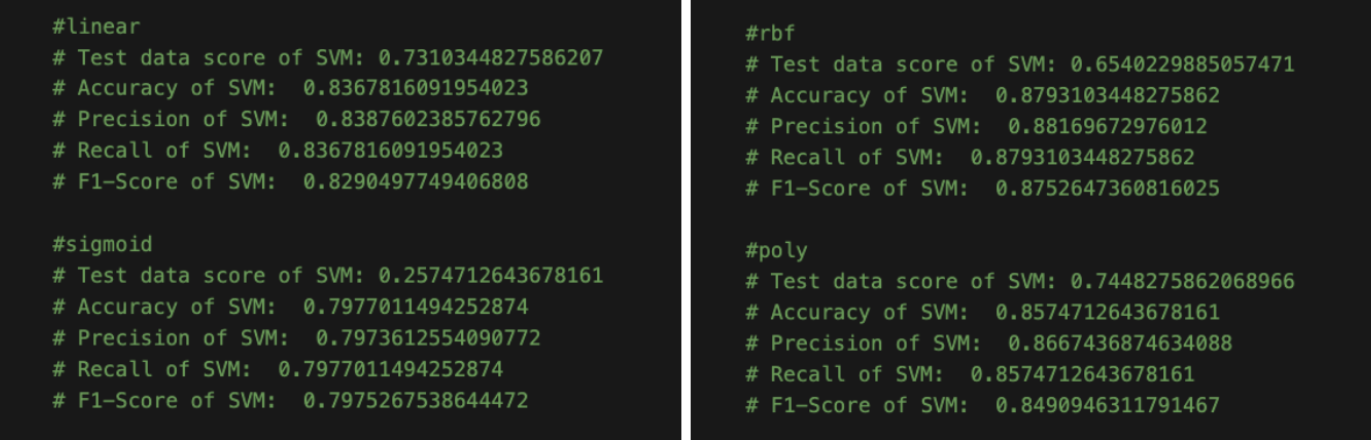
\includegraphics[width=\linewidth]{figures/svm-kernels-and-evaluation-metrics}
%  \caption{SVM Kernels and Evaluation Metrics.}
%\end{figure}

\begin{table}[hbt!]
   \large
   \centering
   \begin{tabular}{lccr}
   \hline
   \textbf{Kernel} & \textbf{Evaluation Metric} & \textbf{Value} \\ 
   \hline
   linear & Test data score & 0.7310344827586207  \\
          & Accuracy & 0.8367816091954023  \\
          & Precision & 0.8387602385762796 \\
          & Recall & 0.8367816091954023  \\
          & F1-Score & 0.8290497749406808  \\
   \hline
   sigmoid & Test data score & 0.2574712643678161  \\
          & Accuracy & 0.7977011494252874  \\
          & Precision & 0.7973612554090772 \\
          & Recall & 0.7977011494252874  \\
          & F1-Score & 0.7975267538644472  \\
   \hline   
   rbf & Test data score & 0.6540229885057471  \\
          & Accuracy & 0.8793103448275862  \\
          & Precision & 0.88169672976012 \\
          & Recall & 0.8793103448275862  \\
          & F1-Score & 0.8752647360816025  \\
   \hline   
   poly & Test data score & 0.7448275862068966  \\
          & Accuracy & 0.8574712643678161  \\
          & Precision & 0.8667436874634088 \\
          & Recall & 0.8574712643678161  \\
          & F1-Score & 0.8490946311791467  \\
   \hline
   \end{tabular}
   \caption{SVM Kernels and Evaluation Metrics.} 
%   \label{tab:example}
\end{table}

\subsubsection{Model Evaluation}
Another way that we can evaluate our SVM classification model on unseen data is to use K-Folds cross-validation. This technique involves dividing the available data into multiple folds (subsets), using one fold for validation/test set and the remaining folds for training the model. The process is repeated K times where each time a different fold is used for the validation set. Results from each validation step are then averaged. This technique provides more than one test/train split of the input data, and provides a more robust estimate of the model’s performance. It divides the data into multiple folds and trains the SVM model on each fold while testing on the others. \cite{geekforgeeks2023}

The main purpose of cross-validation is to help prevent overfitting of the trained subset data to the model. New unseen data from our validation set could perform poorly on the model producing invalid predictions if the trained subset fit too well to the model. Good results from cross-validation will ensure that the model is robust and generalizes well to new data. \cite{geekforgeeks2023}

Testing with our SVM model we chose a 30\% validation set and 70\% training subset; having a higher percentage for the training subset will ensure that our input bias is minimized as this will include more relevant input features needed to create a more robust model. Table 3 shows K-Fold cross validation metrics where the mean accuracy of the model gets better (closer to 1) at 4 or 5 folds. With the SVM model with kernel=’rbf’ and the one pass train/test split, we generated an accuracy of 0.879 which is better than the 4 or 5 fold results but they are similar to show that the model is robust. Setting K-Folds higher than 5, we didn’t notice the mean accuracy change much.

%\end{multicols}

%\begin{figure}[h]
%  \centering
%  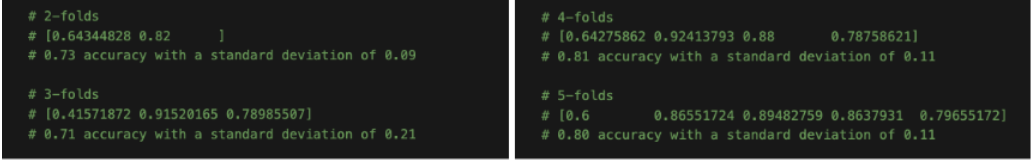
\includegraphics[width=\linewidth]{figures/k-fold-cross-validation-metrics}
%  \caption{K-Fold Cross Validation Metrics.}
%\end{figure}

\begin{table}[hbt!]
   \large
   \centering
   \begin{tabular}{lccr}
   \hline
   \textbf{N-Folds} & \textbf{Scores} & \textbf{Evaluation Metrics} \\ 
   \hline
   2 & \multicolumn{1}{l}{[0.64 0.82]} & 0.73 accuracy with a standard deviation of 0.09 \\
   3 & \multicolumn{1}{l}{[0.42 0.92 0.79]} & 0.71 accuracy with a standard deviation of 0.21 \\
   4 & \multicolumn{1}{l}{[0.64 0.92 0.88 0.79]} & 0.81 accuracy with a standard deviation of 0.11 \\
   5 & \multicolumn{1}{l}{[0.60 0.87 0.89 0.86 0.80]} & 0.80 accuracy with a standard deviation of 0.11 \\
   \hline
   \end{tabular}
   \caption{K-Fold Cross Validation Metrics.} 
%   \label{tab:example}
\end{table}

%\end{multicols}

\subsection{Best Model Fit}
We evaluated each model (kNN and SVM) to see which one predicted the 'completed\_task' output best. Figure 6 shows a comparison of prediction results between our SVM and K-Nearest Neighbors on a testing set in the form of confusion matrices. The results of these two models are comparable, where both models performed well at accurately classifying if a task was not completed. One noteworthy difference between the two models is that the SVM was able to identify more true negative results than the kNN model, where it could correctly classify 30 more uncompleted tasks than the kNN model. On the other hand, it mistakenly classified about 50 more tasks as incomplete than the kNN model. So, overall, our SVM could be seen as more “pessimistic” than the kNN model, since it will tend to classify more tasks as incomplete.

\begin{figure}[hbt!]
  \centering
  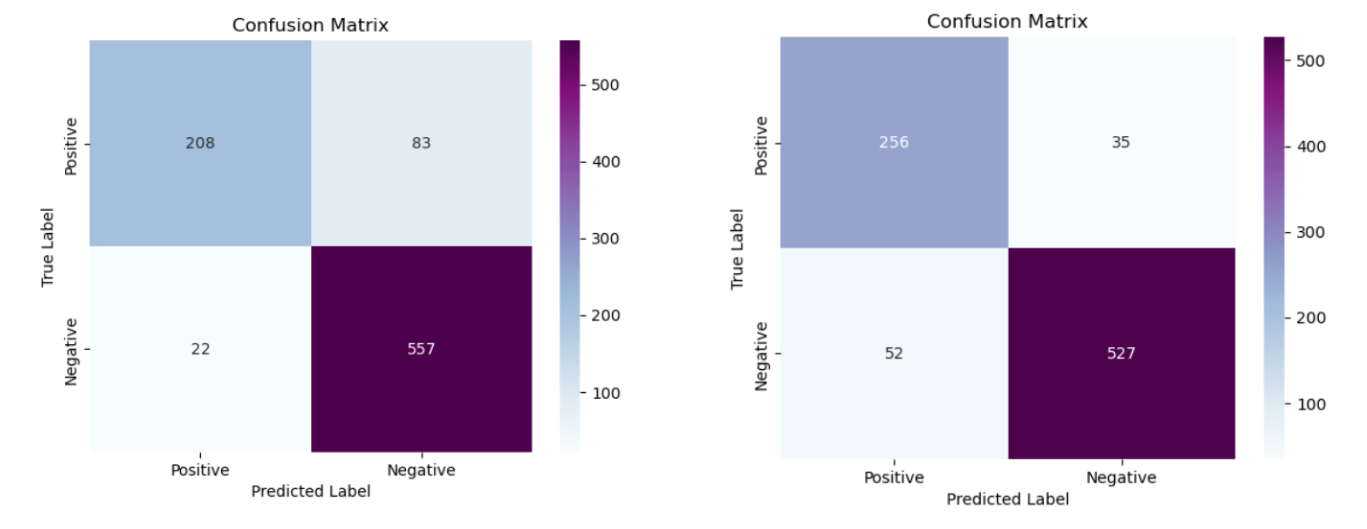
\includegraphics[width=\linewidth]{figures/confusion-matrices-svm-knn}
  \caption{Confusion Matrices: Support Vector Machine (left), K-Nearest Neighbors (right).}
\end{figure}

\pagebreak

\subsection{Predictions for Cases of Interest}
With cases of interest, we were interested to see how the SVM model would predict 3 new cases of interest based on the following variables: high monetary reward, high assignable HIT counts, and a high labor event count. These are the results we found when examining it.

\subsubsection{Case 1: High Monetary Reward}
We can see a high amount of monetary rewards (in dollars) offered, along with a low amount of assignable hits and 158 total labor events that occurred within this case. As we can see this task was completed, which our model correctly predicted.

\begin{lstlisting}[language=Python, caption=Case 1 - Feature input and 'completed\_task' ouptut.]
# ['task.monetary_reward_in_dollars', 'task.assignable_hits_count', 'total.labor.event_count']
case1 = [0.65, 0.0, 158]
case1Result = [1]
\end{lstlisting}

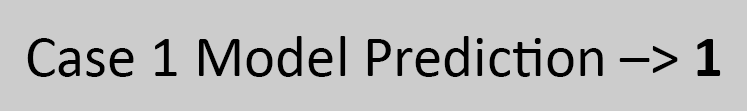
\includegraphics[width=0.35\textwidth, center]{figures/case-1-model-prediction}

\subsubsection{Case 2: High Assignable Hits Count}
We can see a high amount of assignable hits count offered, along with \$0.08 of monetary reward and 234 total labor events that occurred within this case. As we can see this task was completed, which our model correctly predicted.

\begin{lstlisting}[language=Python, caption=Case 2 - Feature input and 'completed\_task' ouptut.]
# ['task.monetary_reward_in_dollars', 'task.assignable_hits_count', 'total.labor.event_count']
case1 = [0.08, 5083.0, 234]
case1Result = [1]
\end{lstlisting}

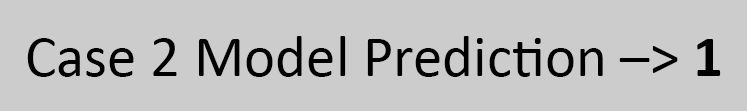
\includegraphics[width=0.35\textwidth, center]{figures/case-2-model-prediction}

\subsubsection{Case 3: High Total Labor Event Count}
We can see a high amount of total labor events occur, along with 0.0 amount of assignable hits and 705 total labor events. As we can see this task was not completed, which our model correctly predicted.

\begin{lstlisting}[language=Python, caption=Case 3 - Feature input and 'completed\_task' ouptut.]
# ['task.monetary_reward_in_dollars', 'task.assignable_hits_count', 'total.labor.event_count']
case1 = [0.08, 0.0, 705]
case1Result = [0]
\end{lstlisting}

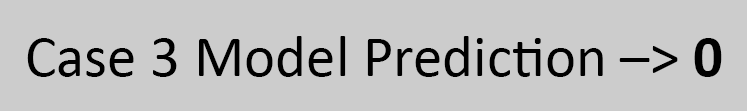
\includegraphics[width=0.35\textwidth, center]{figures/case-3-model-prediction}

\pagebreak

\section{Summary and Conclusion}
TBD


% THE DOCUMENT IS ESSENTIALLY DONE AT THIS POINT, NO NEED TO EDIT ANYTHING BELOW THIS______________________________________________________________________________________________

\bibliographystyle{alpha}
\bibliography{bibliography}

\end{document}